\documentclass[tikz,border=2pt]{standalone}
\usepackage{amsmath}
\usetikzlibrary{arrows.meta}
\begin{document}
% Survival and deferred death events for a life aged 40: {}_5p_{40} = P(T_40 > 5) = 0.98,
% {}_{10}p_{40} = P(T_40 > 10) = 0.95, and {}_{5|5}q_{40} = P(5 < T_40 <= 10) = 0.98 - 0.95 = 0.03.
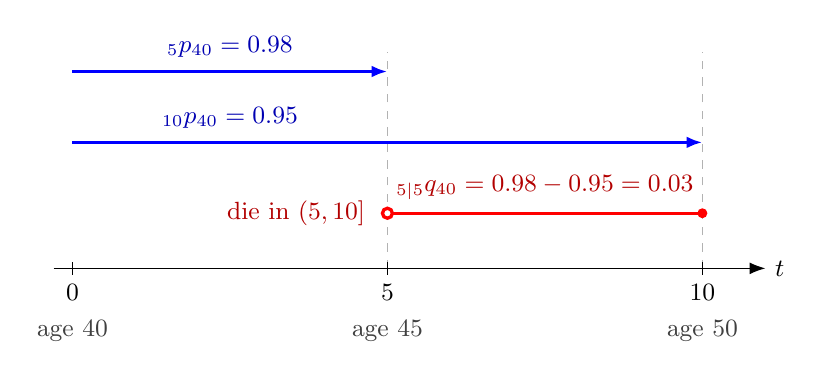
\begin{tikzpicture}[font=\small, >={Latex[length=2mm]}, x=0.8cm, y=1cm]
  \draw[gray!60, thin, dashed] (5,0) -- (5,2.75);
  \draw[gray!60, thin, dashed] (10,0) -- (10,2.75);
  \draw[->] (-0.3,0) -- (11.0,0) node[right] {$t$};
  \foreach \k/\a in {0/40,5/45,10/50} {
    \draw (\k,0.08) -- (\k,-0.08) node[below] {$\k$};
    \node[gray!50!black] at (\k,-0.8) {age $\a$};
  }
  % survive to t = 5
  \draw[blue, very thick, -{Latex[length=2mm]}] (0,2.5) -- (5,2.5);
  \node[blue!70!black, anchor=south] at (2.5,2.55) {${}_5p_{40}=0.98$};
  % survive to t = 10
  \draw[blue, very thick, -{Latex[length=2mm]}] (0,1.6) -- (10,1.6);
  \node[blue!70!black, anchor=south] at (2.5,1.65) {${}_{10}p_{40}=0.95$};
  % die in (5,10]
  \draw[red, very thick] (5,0.7) -- (10,0.7);
  \draw[red, very thick, fill=white] (5,0.7) circle (1.8pt);
  \fill[red] (10,0.7) circle (1.8pt);
  \node[red!70!black, anchor=south] at (7.5,0.75) {${}_{5|5}q_{40}=0.98-0.95=0.03$};
  \node[red!70!black, anchor=east] at (4.8,0.7) {die in $(5,10]$};
\end{tikzpicture}
\end{document}
